\chapter{Combining React and D3}
\label{cha:visualization}

The most important aspect of the master's thesis is the thesis project. This chapter introduces the reader to the project implementation and the resulting prototypes that were developed during the development phase of the thesis project. A complete walk-through helps the reader to understand the implementation differences of all prototypes. Finally, the chapter introduces the reader to the performance testing methodology and the different devices that were used to benchmark the prototypes.

\section{Introduction and Motivation of the Project}

When trying to find the best combination of two libraries, developing prototypes is extremely important. Combining \emph{React} and \emph{D3} in a few different ways in the thesis project ultimately lead to one prototype that then came out on top. The project was primarily realized to provide \emph{React} developers with an alternative to native \emph{D3} force implementations. The resulting software makes it possible to use \emph{D3's} force simulations by writing \emph{React} code. Finding a \emph{React} implementation of \emph{D3's} force simulation which performs better than the native \emph{D3} implementation was not the primary goal of the project.

The obvious question "Why do I even need a combination of \emph{React} and \emph{D3} if I could just use native \emph{D3} instead?" can quickly be answered. The initial idea of the project came to mind when a client requested a fully fledged \emph{React} web application, which also included some complex data visualization aspects that have to be animated in the browser. Instead of implementing the visualization part of the application in native \emph{D3}, the combination of \emph{React} and \emph{D3} enables all developers of the project to write declarative \emph{React} code. Using a combination layer API results in only one code base that has to be maintained, instead of two. Also, as mentioned before, \emph{D3} code bases tend to become exponentially more challenging to maintain as the project grows.

\section{Project Setup}
\label{sub:projectSetup}

\begin{program}
\caption{Simple example of a \emph{React} component and its usage.} 
\label{prog:forceBuildModule}
\begin{JsCode}
const applyForceHandlers = pipeAppliers( /+\label{line:composition1}+/
  applyGeneralForce, 
  applyLinkForce, 
  applyCollisionForce
)

const applyEndHandlers = pipeAppliers( /+\label{line:composition2}+/
  applyOnEndHandler, 
  applySimulationReheating
)

const pureD3Updater = pipeAppliers( /+\label{line:updater1}+/
  applyNewNodeData,
  applyPureD3Selection, /+\label{line:applyPureD3Selection}+/
  applyTickHandler,
  applyForceHandlers, /+\label{line:applyForce1}+/
  applyDragHandlers,
  applyEndHandlers,
)

const hybridUpdater = pipeAppliers( /+\label{line:updater2}+/
  applyNewNodeData,
  applyNewRefs, /+\label{line:applyNewRefs}+/
  applyTickHandler,
  applyForceHandlers, /+\label{line:applyForce2}+/
  applyDragHandlers,
  applyEndHandlers,
)

const pureReactUpdater = pipeAppliers( /+\label{line:updater3}+/
  applyNewNodeData, 
  applyForceHandlers, /+\label{line:applyForce3}+/
  applyEndHandlers
)

const getUpdaterFunction = switchCase({ /+\label{line:getUpdaterFunction}+/
  [SIMULATION_TYPE.PURE_D3]: pureD3Updater,
  [SIMULATION_TYPE.REACT_D3_HYBRID]: hybridUpdater,
  [SIMULATION_TYPE.PURE_REACT]: pureReactUpdater,
})(null)

export const buildForceSimulation = (options) => { /+\label{line:buildForceSimulationFn}+/
  const simulation = forceSimulation()
  const updateSimulation = getUpdaterFunction(options.type)
  updateSimulation({ simulation, options })
  return { simulation, updateSimulation }
}
\end{JsCode}
\end{program}

\afterpage{\clearpage}

To be able to test multiple prototypes, one crucial aspect of the project is the force simulation builder setup. All prototypes are based on the simulation builder module which contains a few \emph{D3} specific methods that allow developers to construct their own individual force simulation variants. The prototypes can reuse some of the already composed methods, and some new custom methods can be implemented as well.

By implementing a force simulation builder module, it is possible to ensure that all prototype \emph{D3} simulations are initialized and updated the same way. The most interesting code snippet of the module can be seen in program~\ref{prog:forceBuildModule}. Individual building blocks of the simulation can be piped together because the module uses a functional approach. Lines~\ref{line:updater1},~\ref{line:updater2} and~\ref{line:updater3} show how the updater functions for the three prototypes are composed together by using smaller force simulation function blocks.

The \texttt{buildForceSimulation()} method in line~\ref{line:buildForceSimulationFn} in program~\ref{prog:forceBuildModule} is the most important function in the module. The options parameter has to contain a type, which is used to determine what updater function is applied to the force simulation. The functional switch case statement on line \ref{line:getUpdaterFunction} in program~\ref{prog:forceBuildModule} decides based on the type which updater function to return. The builder function returns an instance of a \emph{D3} force simulation and the associated updater function that can be used by each prototype to update the simulation every time the data changes.

Another interesting aspect of the code snippet in program~\ref{prog:forceBuildModule} is that the functional compositions can be nested. Lines~\ref{line:composition1} and~\ref{line:composition2} show the composition of two functions that in turn can then be composed with all three force simulation variants. Even though they are piped together, the result can then be piped again into every updater function composition as shown in lines~\ref{line:applyForce1},~\ref{line:applyForce2}, and~\ref{line:applyForce3}, for example, where the composed method \texttt{applyForceHandlers} is piped into the updater functions of the different prototypes. Again, the way the updater function composition is implemented ensures the equality of the force simulation initialization of all three prototypes.

Of course, since all three prototypes work fundamentally different, some custom apply functions have to be implemented to ensure the functionality of all three prototypes. Applying the custom functions is no problem, as all updater functions are functional compositions. If some custom method has to be added, it can just be applied to the function composition of the associated prototype. Line~\ref{line:applyNewRefs} in program~\ref{prog:forceBuildModule} shows how a custom node reference applying function is composed into the updater function.

Each prototype implements the same API interface and receives its data via props. All visualization data and every setting parameter, therefore, has to be passed to the prototype component via \emph{React} component props. Using props also means that the data and the settings must be updateable. The parent container which renders a prototype component must be able to update the prototype's data by just passing different props. The newly applied props, as a consequence, have to be handled correctly in each prototype individually.

%% DATA ENCAPSULATION %%

\section{Prototypes}

This section introduces the reader to the prototypes of the thesis project. It also explains how the project initially originated. Furthermore, every resulting prototype of the project is listed and explained extensively. All in all, the thesis project yielded three viable prototypes that are described in this chapter. 

%% ----------------------------------------------------------------------------------------- %%
%% ---------------------------------------- PURE D3 ---------------------------------------- %% 
%% ----------------------------------------------------------------------------------------- %%

\subsection{Pure D3 Prototype}
\label{sec:pureD3prototype}

\begin{figure}
\centering
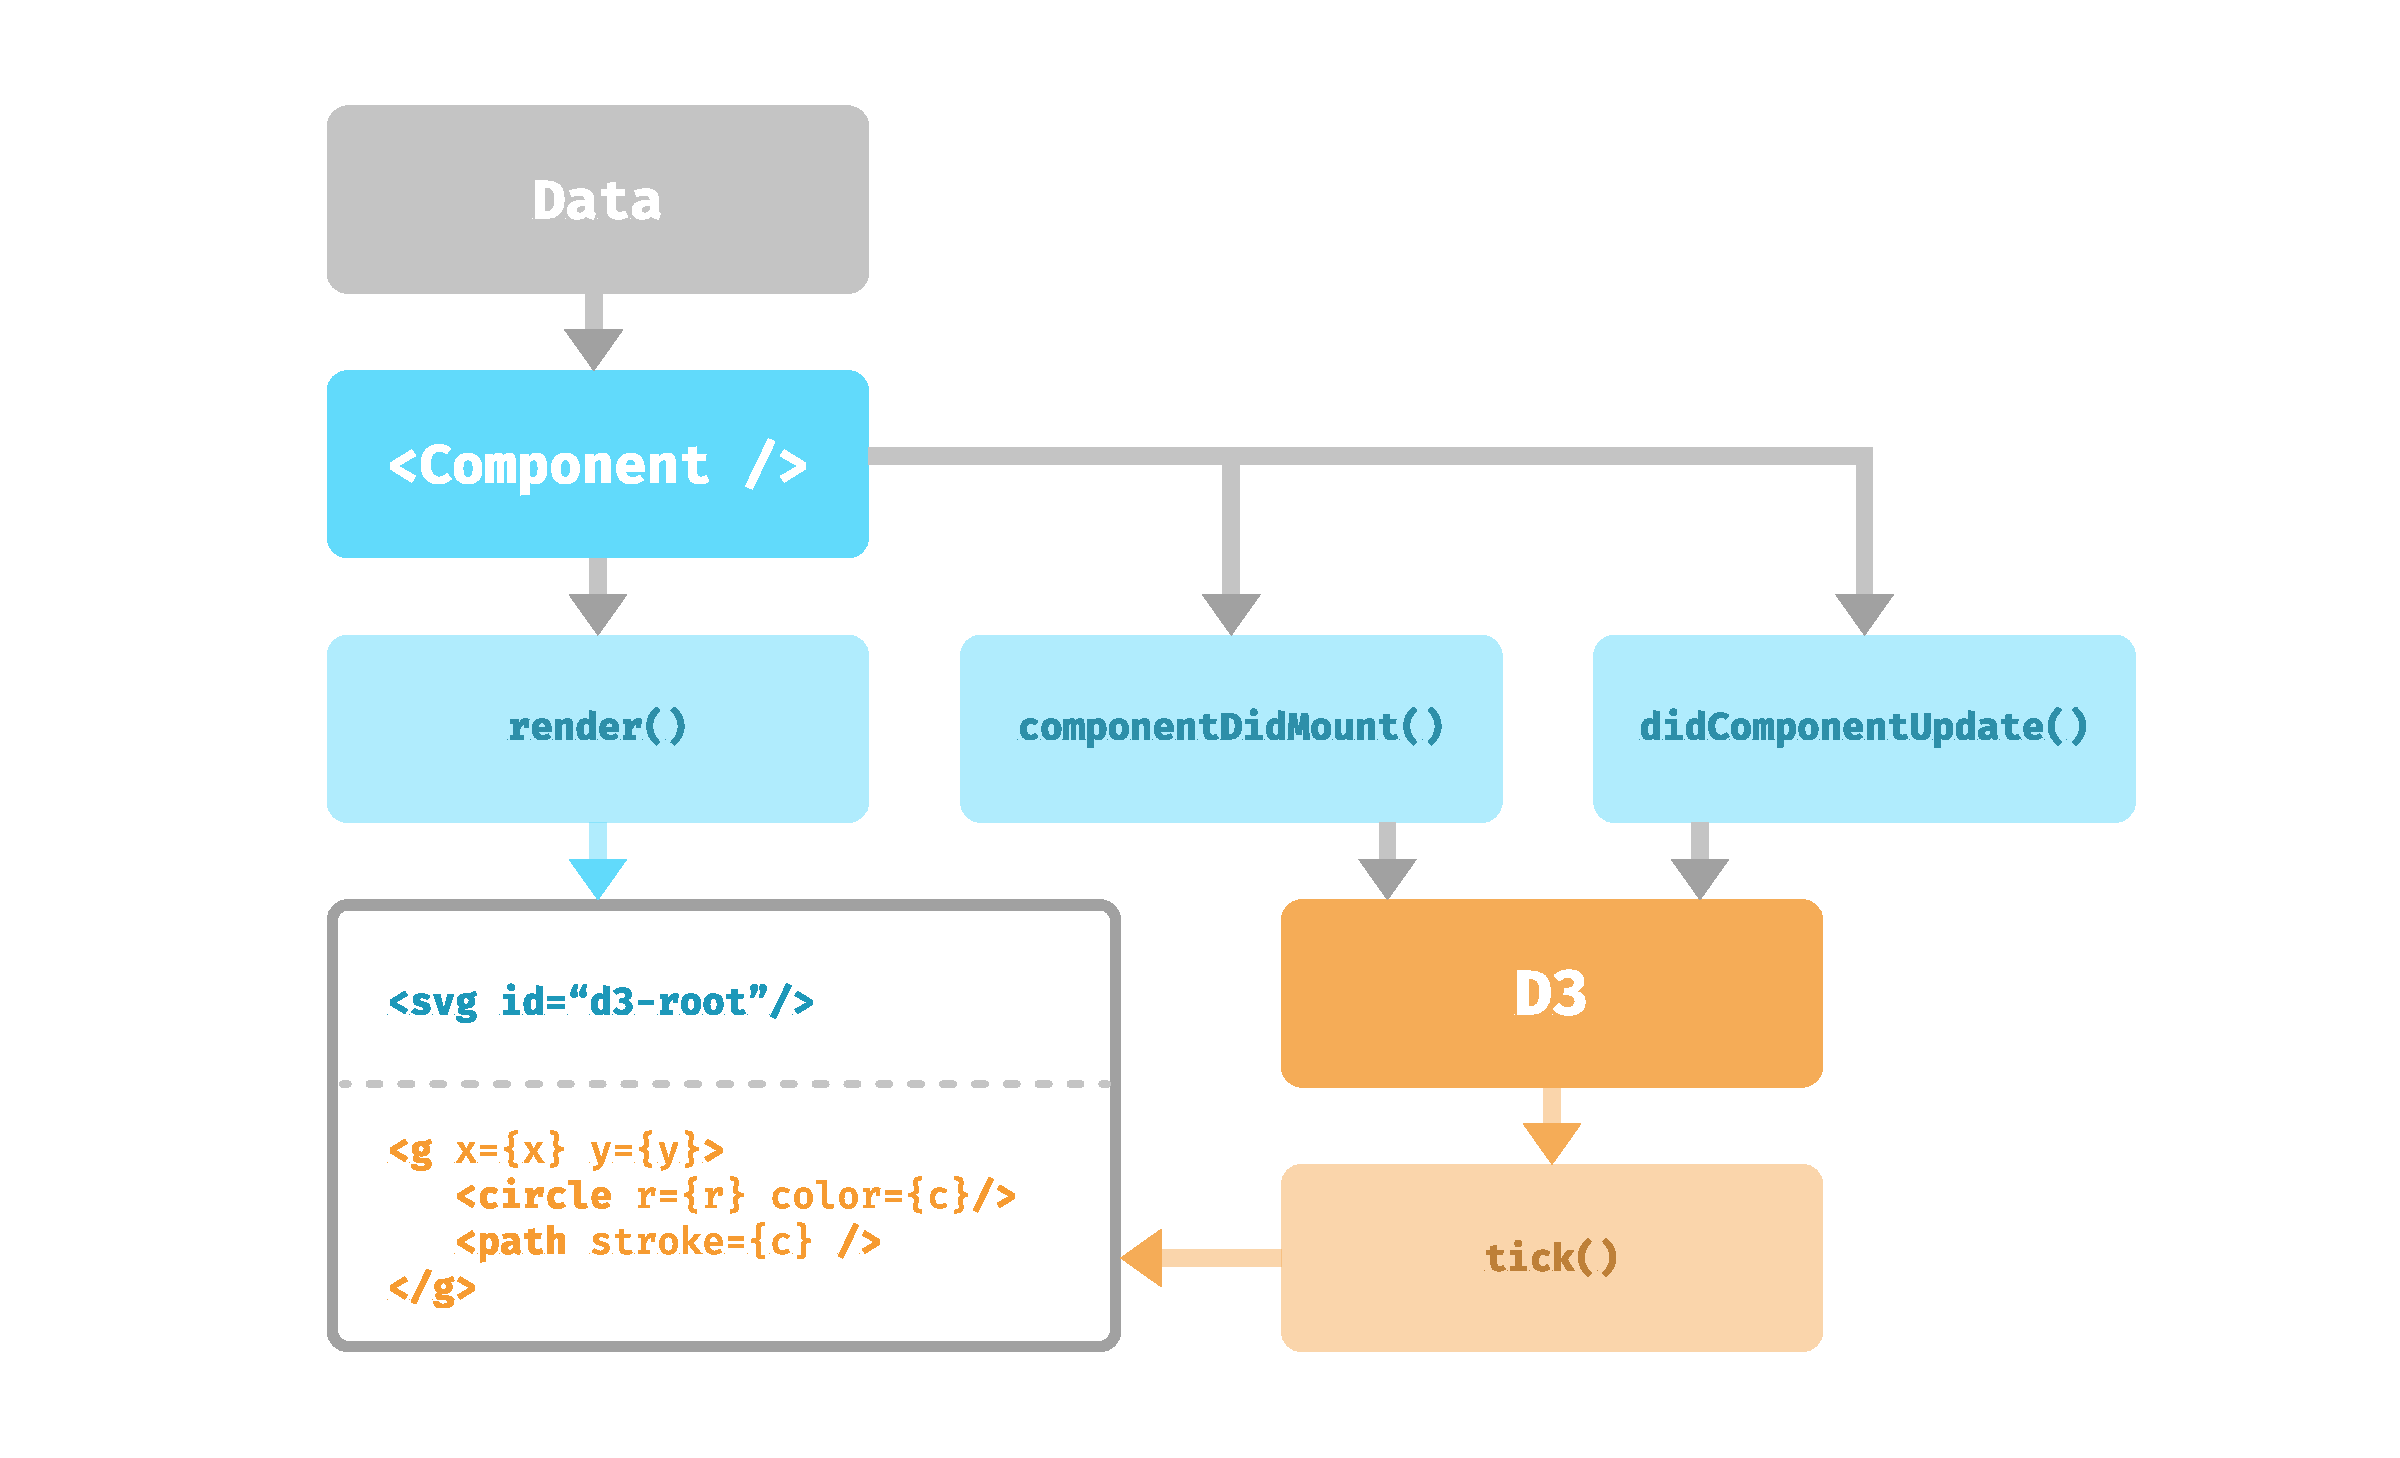
\includegraphics[scale=.6, trim= 4cm 0 4cm 0, clip, width=0.85\columnwidth]{impl001.pdf}
\caption{Pure \emph{D3} force graph life cycle visualization.}
\label{fig:pureD3Lifecycle}
\end{figure}

The first prototype of the project was developed from an early experimental implementation. The sole reason it was realized was to test if it is even possible to combine \emph{React} and \emph{D3} but still maintaining \emph{React's} philosophy of unidirectional dataflow and idempotent render function components. The main goal, therefore, was to create a prototype that would always correctly update itself and thus visualize current data props on every render cycle. If the parent component updated the visualization component's data or options, the prototype would have to instantly reflect the changes as well. The main difficulty with this prototype is to combine \emph{React's} declarative approach with \emph{D3's} imperative way of rendering data.

The implementation heavily relies on the fact that \emph{React's} reconciliation algorithm omits updates to the DOM if the same element is rendered consecutively. The pure \emph{D3} graph component renders a single static base SVG, as shown in the code snippet in program~\ref{prog:pureD3render}. After the component mounts, \emph{D3} hooks into the base SVG component via the provided reference to the actual base DOM node and builds its force simulation on top. \emph{D3} also appends and removes the DOM nodes according to the data that was passed to \emph{D3}. Figure~\ref{fig:pureD3Lifecycle} demonstrates via color coding how \emph{React} only renders the SVG element and \emph{D3} renders the simulation via the tick function.

\begin{program}
\caption{Render function of the pure \emph{D3} prototype.}
\label{prog:pureD3render}
\begin{JsCode}
render() {
  const { width, height } = this.props
  return <svg ref={this.ref} width={width} height={height} />
}
\end{JsCode}
\end{program}

As a result, \emph{React's} reconciliation algorithm does not handle nodes that are inside the \emph{D3} force simulation if the data changes. The component only renders a static SVG element that is not updated. Because the SVG element is static, \emph{React's} reconciliation algorithm does not commit anything to the DOM since every time the render function is called the SVG tag stays the same. Instead, \emph{D3} entirely takes over the DOM manipulation and adequately handles the simulation by itself without \emph{React} interfering in any way.

Every time the data updates, the new data is provided directly to \emph{D3} via the life cycle method \texttt{componentDidUpdate()} as figure~\ref{fig:pureD3Lifecycle} shows. Of course, every data update causes \emph{React} to render the base SVG component, but, due to the virtual DOM implementation of \emph{React}, the SVG is never newly rendered, as it never changes. A static component is a \emph{React} node that does not contain any dynamic content and is therefore never updated by the reconciliation phase. \emph{React's} reconciliation algorithm prevents the browser from newly committing the SVG tag to the DOM. \emph{D3}, therefore, works completely separate from \emph{React}. \emph{D3}, on the other hand, can be implemented like in any other native \emph{D3} web project. Not only the initial force graph generation functionality has to be implemented but also the update logic that handles the updated data and applies it to the force graph simulation.

There are two component life cycle methods from \emph{React} that are crucial to this implementation. First, \texttt{componentDidMount()} is used to initialize \emph{D3}, select the base node, and then build the whole force simulation on top as demonstrated in program~\ref{fig:pureD3Lifecycle}. It is important to use the life cycle method that triggers \emph{after} the initial commit phase, as it makes sure, the component has already been rendered once for \emph{D3} to being able to select the existing real SVG DOM node. Looking at figure~\ref{fig:pureD3Lifecycle} again, it is apparent that the second important life cycle method is \texttt{componentDidUpdate()} which provides the latest most up to date data directly to \emph{D3}. That way \emph{D3} can handle the update in the force graph.

\subsubsection{Implementation Details}

Once the component is initialized, the \texttt{componentDidMount()} life cycle method directly calls the initializer function which can be seen on line~\ref{line:initGraphFn} in the code snippet in program~\ref{prog:pureD3InitFn}. The initializing function appends the base \texttt{<g>} tag and also handles the translation of the current height and width of the component. Then the \texttt{build\-Force\-Simulation()} function is called with the current options and parameters in order to get the simulation and the correct updater function. Note how the simulation type is passed to the builder function as well. The resulting simulation and updater function is then saved in the current component.

\begin{program}
\caption{Pure \emph{D3} force graph initializing function.}
\label{prog:pureD3InitFn}
\begin{JsCode}
initGraph = () => { /+\label{line:initGraphFn}+/
  const { width, height, onSimulationStart } = this.props

  onSimulationStart()

  const svg = select(this.ref.current)
  svg
    .append('g')
    .attr('transform', 'translate(' + width / 2 + ',' + height / 2 + ')')

  const simOptions = this.extractSimOptions()
  const { simulation, updateSimulation } = buildForceSimulation({ /+\label{line:buildForceSimulation}+/
    type: SIMULATION_TYPE.PURE_D3,
    ...simOptions,
  })

  this.simulation = simulation /+\label{line:thisContext1}+/
  this.updateSimulation = updateSimulation /+\label{line:thisContext2}+/
}
\end{JsCode}
\end{program}

What is also worth mentioning is the fact that the simulation and the updating functions are saved directly to the \texttt{this} context as seen in lines~\ref{line:thisContext1} and~\ref{line:thisContext2} of the code snippet in program~\ref{prog:pureD3InitFn}. As stateful components are just plain \emph{JavaScript} classes, they are capable of having member variables as well. It is of utmost importance not to confuse member variables with \emph{React's} component state, as \emph{React} is agnostic to class member variables. \emph{React} not noticing the member variables is a desired effect in this case, as the simulation and the updater function have to be saved in the component without \emph{React} going through a new render cycle. 

Looking at the code in program~\ref{prog:pureD3updateApply}, the update applying functionality can be seen very well. If given a current simulation object, the function handles all newly entering, transitioning, and exiting nodes accordingly. Even an animation is applied. Each time, the pure \emph{D3} \emph{React} component goes through the \texttt{componentDidUpdate()} function, the \texttt{applyNodeUpdateCycle()} function is called as well. The force simulation building module can take in the updater function from the example in program~\ref{prog:pureD3updateApply} and composes it directly into the updating function as seen in line~\ref{line:applyPureD3Selection} in program~\ref{prog:forceBuildModule}.

\begin{program}[th]
\caption{Function that applies the data update to \emph{D3} on data changes.}
\label{prog:pureD3updateApply}
\begin{JsCode}
applyNodeUpdateCycle = (simulation) => {
  simulation.linkSel.exit().remove()
  
  simulation.linkSel = simulation.linkSel
    .enter()
    .append('path')
    .attr('stroke', '#45b29d')
    .attr('fill', 'none')
    .merge(simulation.linkSel)
  
  let t = transition().duration(750)
  
  simulation.nodeSel
    .exit()
    .style('fill', '#b26745')
    .transition(t)
    .attr('r', 1e-6)
    .remove()
  
  simulation.nodeSel
    .transition(t)
    .style('fill', '#3a403d')
    .attr('r', ({ size }) => size)
  
  simulation.nodeSel = simulation.nodeSel
    .enter()
    .append('circle')
    .style('fill', '#45b29d')
    .attr('r', ({ size }) => size)
    .attr('id', ({ name }) => name)
    .merge(simulation.nodeSel)
}
\end{JsCode}
\end{program}

Another vital function of the pure \emph{D3} force graph is the tick handler that can be seen in program~\ref{prog:pureD3Tick}. The ticking function also gets passed to the force simulation builder function. Each iteration of \emph{D3's} simulation tick the function updates the position of all nodes and links in the simulation.

\begin{program}[th]
\caption{Tick handling function of the pure \emph{D3} prototype.}
\label{prog:pureD3Tick}
\begin{JsCode}
ticked = () => {
  this.simulation.nodeSel.attr('cx', ({ x }) => x).attr('cy', ({ y }) => y)
  this.simulation.linkSel.attr('d', (d) =>
    this.props.linkType === LINK_TYPES.CURVED ? getCurvedLinkPath(d) : getStraightLinkPath(d),
  )
}
\end{JsCode}
\end{program}

\subsubsection{Advantages}

One of the most apparent advantages of the pure \emph{D3} force graph implementation is its performance, of course. Since the implementation uses a native \emph{D3} approach to render and update the nodes and links in the simulation, the performance is also comparable to a native \emph{D3} implementation. In chapter~\ref{cha:performance}, the performance of the pure \emph{D3} prototype is compared to the other implementations.

\subsubsection{Disadvantages}

The most sig\-nifi\-cant disadvantage of the pure \emph{D3} implementation is the fact that all DOM manipulations are handled via imperatively chained function calls on the node selections of \emph{D3} which also implies that the node rendering functionality cannot be customized by passing custom render functions for instance. The force graph's code itself has to be changed to get different node and link appearances, which leads to the previously described problem of encountering unmaintainable code over time.

%% ---------------------------------------------------------------------------------------- %%
%% -------------------------------------- PURE REACT -------------------------------------- %% 
%% ---------------------------------------------------------------------------------------- %%

\subsection{Pure React Prototype}
\label{sec:pureReactPrototype}

\begin{figure}
\centering
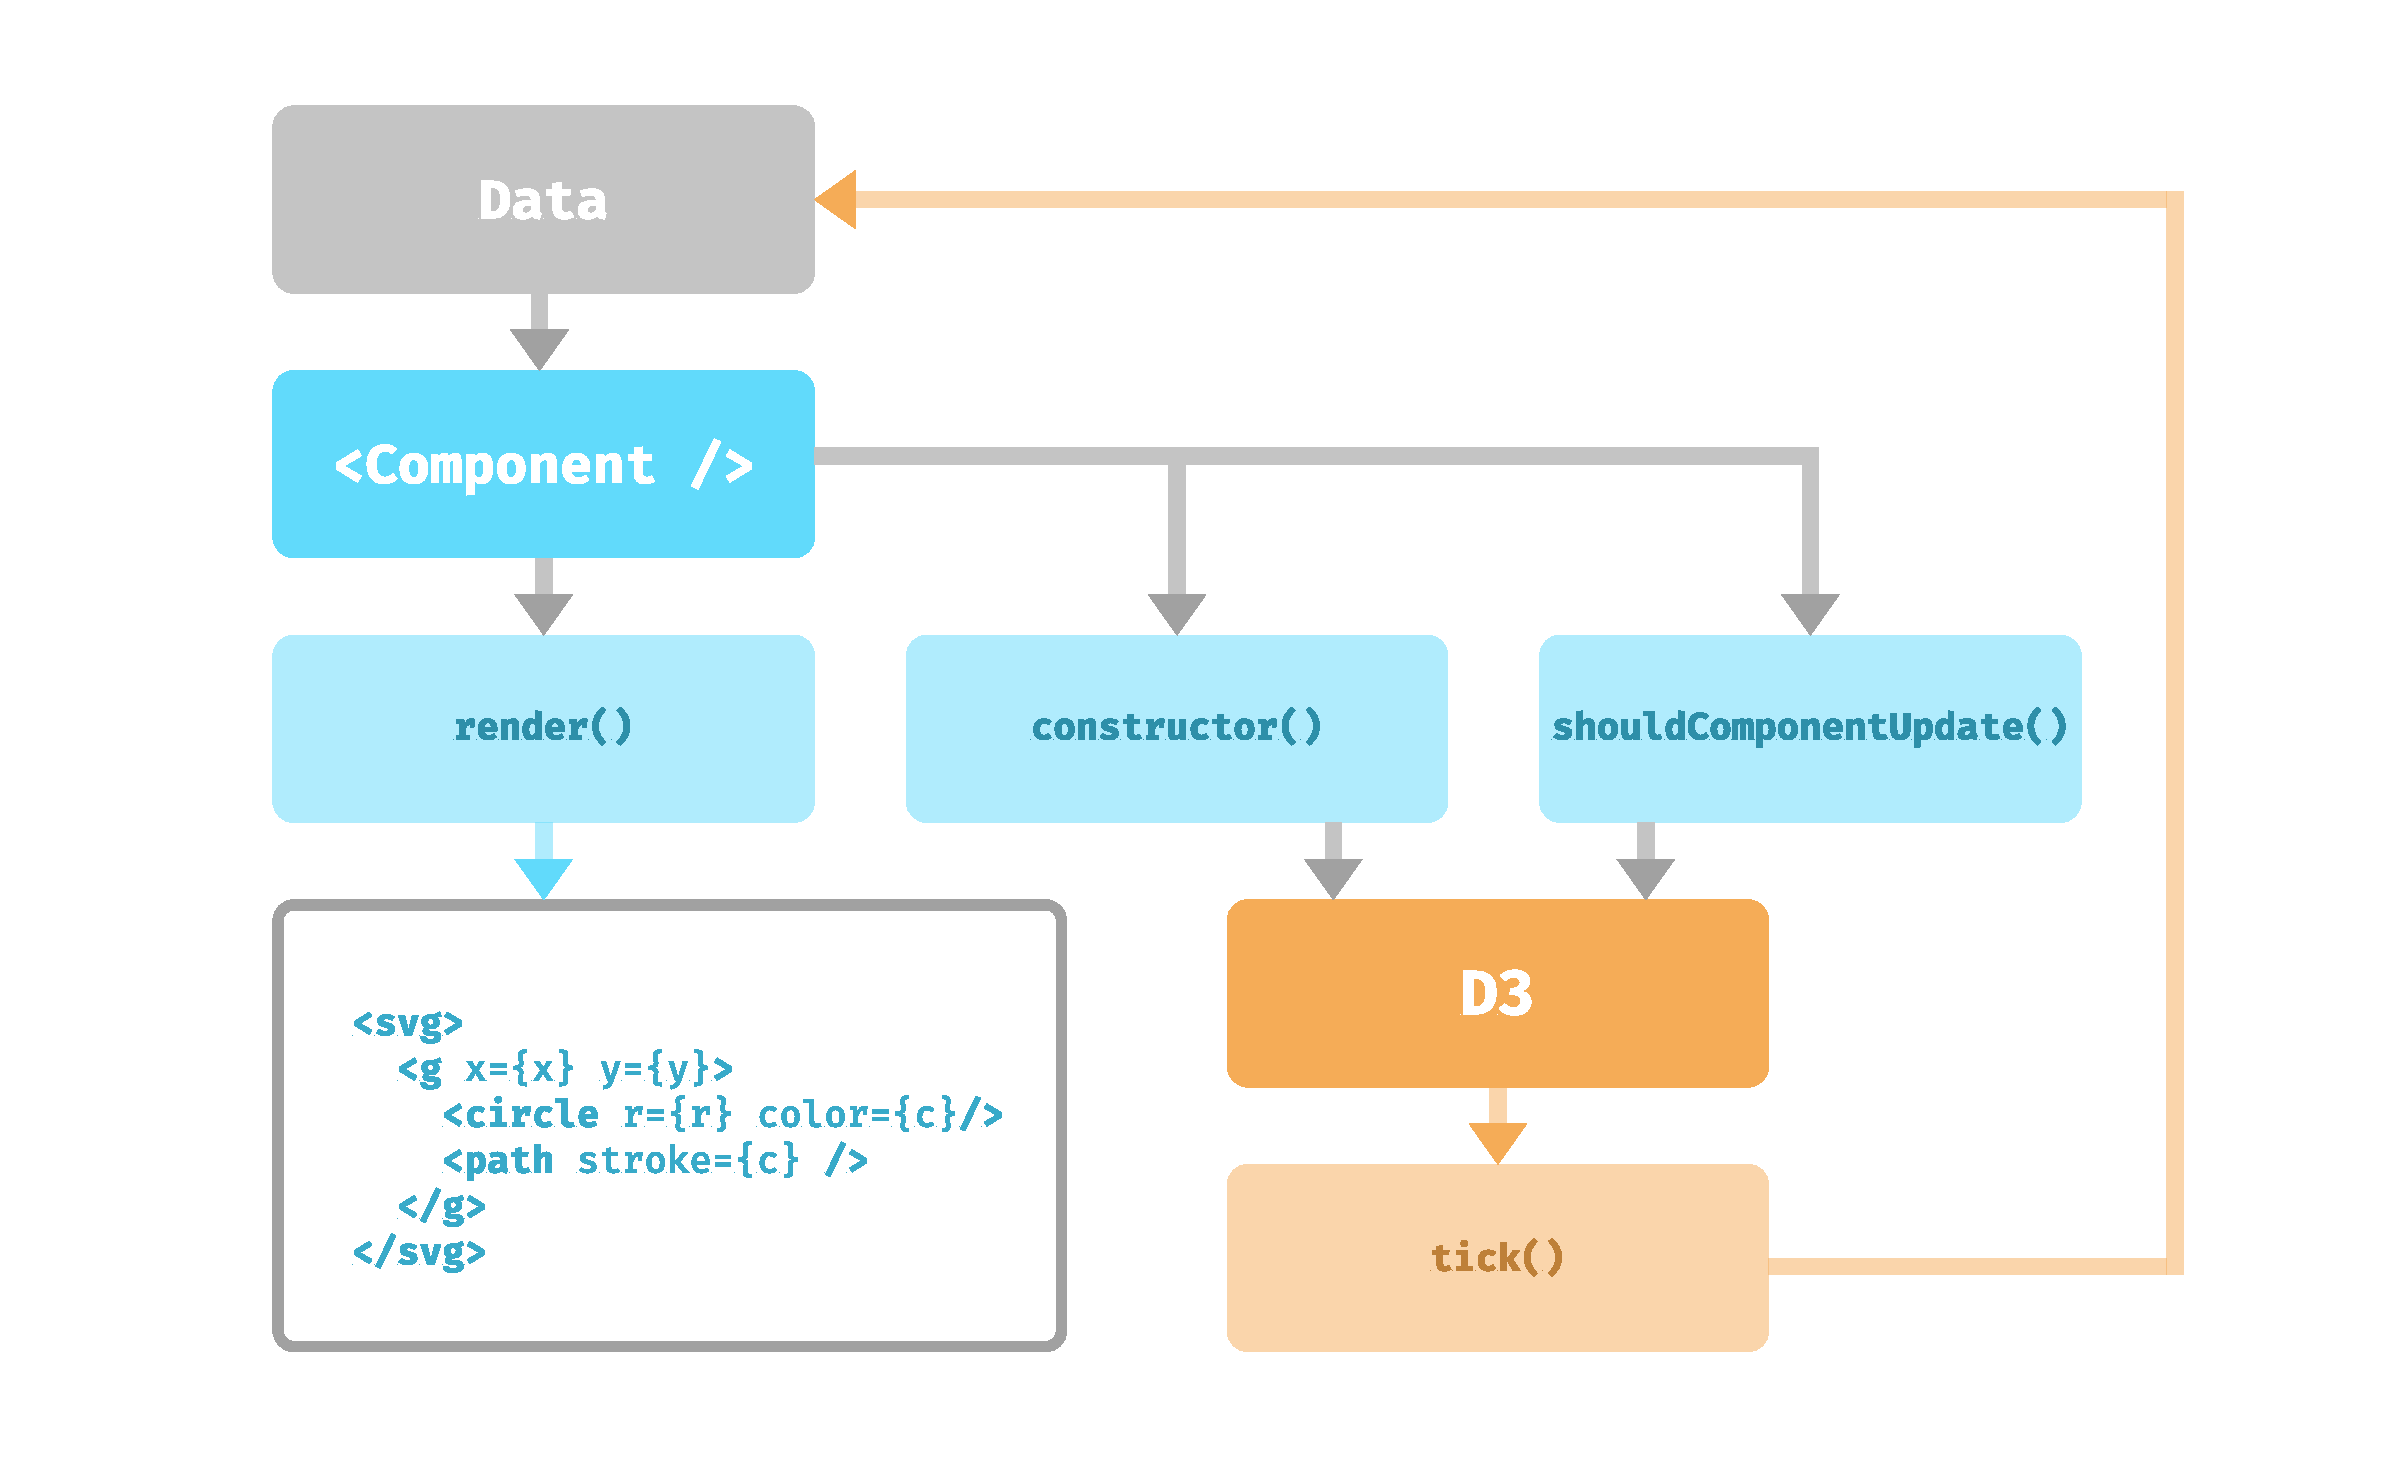
\includegraphics[scale=.6, trim= 4cm 0 2cm 0, clip, width=0.85\columnwidth]{impl002.pdf}
\caption{Pure \emph{React} force graph life cycle visualization.}
\label{fig:pureReactLifecycle}
\end{figure}

The pure \emph{React} force graph implementation is far more complicated than the pure \emph{D3} force graph, as the \emph{D3} implementation is just a \emph{React} wrapper for \emph{D3}. To achieve a pure \emph{React} implementation, \emph{D3} needs to be deeply integrated into the rendering cycle of \emph{React} itself. As mentioned in chapter~\ref{cha:d3js}, \emph{D3} provides developers a tick function when using animated simulations. This tick function is executed as often as the browser has an animation frame available according to \emph{D3's} documentation\footnote{\url{https://github.com/d3/d3-timer}}. Explaining the request animation frame functionality of the browser would go out of the scope of this thesis, but MDN provides a good explanation on the MDN website in~\cite{RAF}.

As figure~\ref{fig:pureReactLifecycle} shows, the complete presentation layer is handled by \emph{React} itself. The whole SVG component tree is completely rendered by \emph{React}. The figure also demonstrates how the data is handled not only in the component's constructor but also in its \texttt{shouldComponentUpdate()} life cycle method. As mentioned in the previous chapter~\ref{cha:react}, the constructor is the first life cycle method that is executed in any \emph{React} component. The pure \emph{React} prototype takes advantage of that fact and initializes the complete \emph{D3} force simulation before any data is rendered. The \texttt{shouldComponentUpdate()} life cycle is used to determine if the component's props have changed and possibly apply an update to the \emph{D3} force simulation.

The key to the integration of \emph{D3} into \emph{React's} render cycle is the tick function on the \emph{D3} force simulation. Every time the tick function is executed, the applied tick handler then queries the force simulation data, fetches all link and node positions, calculates the current position and then passes the newly calculated data to the \emph{React} component again via a \texttt{setState()} call. Figure~\ref{fig:pureReactLifecycle} demonstrates how the data flows back into the component after each tick cycle of the force simulation.

Keeping all node and link positions in the \emph{React} component state, as a result, unlocks full control to the presentation layer. Thus, \emph{React} acting as a function of state can completely handle each element in the force simulation. The component state includes not only appearance properties like background or stroke color but also exact node and link positions. As a consequence, the data has to pass the complete rendering cycle of \emph{React} on every tick execution, including the reconciliation phase, which can lead to poor rendering performance. Not only does it take time for \emph{D3} to calculate a new version of the force data each tick, but also \emph{React} then has to process the whole new data tree. If the simulation contains a high number of nodes, the whole rendering process---which figure~\ref{fig:pureReactLifecycle} shows---should massively impact performance in theory.

An existing project of \emph{Uber}\footnote{\url{https://www.uber.com}} strongly inspired the pure \emph{React} implementation. \emph{Uber's} project is called vis-force and can be found on its git page in~\cite{UberVisForce}. During the research phase of the thesis project, \emph{Uber's} project was found and also thoroughly examined. The pure \emph{React} prototype implementation is essential as it can be used to compare the render performance to the other two prototypes of the thesis project.

\subsubsection{Implementation Details}

The initialization of the pure \emph{React} force graph pretty much looks the same as in line~\ref{line:buildForceSimulation} in the pure \emph{D3} code example in program~\ref{prog:pureD3InitFn}. The pure \emph{React} prototype passes its correct simulation type of course though. The biggest and most important difference to the pure \emph{D3} implementation is that the initialization of the force simulation takes place inside the constructor instead of the \texttt{componentDidMount()} life cycle method. As mentioned before, the pure \emph{React} prototype contains all node and link positions in the internal state. Consequently, the internal state must exist before calling the \texttt{render()} life cycle method the first time.

Due to the fact that the pure \emph{React} force graph component provides the complete dataset about all nodes and links in the simulation, the render function can be 100\% declarative code as seen in the code example in program~\ref{prog:pureReactRender}. The link and node properties which contain presentational data like the size of a node or the color of a link come from the component's props, as they are passed in from the parent container. However, the link and node positions come from the components internal state. The example code in program~\ref{prog:pureReactRender} shows very well, how the nodes and links components have direct access to the link and node positions. Figure~\ref{fig:pureReactLifecycle} also shows how the \emph{React} components handle all the SVG properties.

\begin{program}
\caption{Render life cycle method of the pure \emph{React} force graph prototype.}
\label{prog:pureReactRender}
\begin{JsCode}
render() {
  const { height, width, nodes, links } = this.props
  const { linkPositions, nodePositions } = this.state
  
  return (
    <span style={containerStyle}>
      <svg height={height} width={width}>
        <g style={gStyle} transform={`translate(${width / 2},${height / 2})`}>
          <Links links={links} linkPositions={linkPositions} />
          <Nodes nodes={nodes} nodePositions={nodePositions} />
        </g>
      </svg>
    </span>
  )
}
\end{JsCode}
\end{program}

Another vital aspect of the pure \emph{React} force graph's implementation is the update handling mechanism. Due to the fact that the component is updated on every free animation frame of the browser, it is of utmost importance to only update the component if necessary. The \texttt{shouldComponentUpdate()} function in the code snippet in program~\ref{prog:pureReactSimulationUpdate} shows that not only internal state but also the props are checked, if they have updated. Only if the props provided by the parent component have changed, the component calls the force simulation updater function which it obtained via the \texttt{buildForceSimulation()} call in the constructor. The component should update though if either its props or its state has changed. If the props have changed, the simulation updater function makes sure that the force simulation calculates the data for the new nodes and links. By doing so, the next render call can already process the new node and link positions.

Unfortunately calling the \texttt{handleSimulationUpdate()} function inside \emph{React's} life cycle method \texttt{should\-Component\-Update()} is considered an anti-pattern according to Facebooks article\footnote{\url{https://reactjs.org/docs/react-component.html}}, as side-effects should always be handled inside the \texttt{component\-Did\-Update()} life cycle method. The force simulation updater function is a so-called "side effect." Facebook strongly advises against using any side effects in the \texttt{should\-Component\-Update()} life cycle method, as it should be as fast and efficient as possible to prevent possible render cycles. In the case of the pure \emph{React} force component calling the simulation updater function is fine though, as the side-effect is not called on every state update, but only if the component's props change. Props only change, if the parent component passes different props, which does not happen that often. The internal component state, on the other hand, updates multiple times per second and preventing the simulation update function call on every state change is crucially important for good rendering performance.

\begin{program}
\caption{Update method of the pure \emph{React} force graph prototype.}
\label{prog:pureReactSimulationUpdate}
\begin{JsCode}
shouldComponentUpdate(nextProps, nextState) => {
  const propsChanged = shallowCompare(this.props, nextProps)
  const stateChanged = shallowCompare(this.state, nextState)
  const shouldUpdate = propsChanged || stateChanged
  propsChanged && this.handleSimulationUpdate(nextProps)
  return shouldUpdate
}
\end{JsCode}
\end{program}

Another interesting aspect of the pure \emph{React} prototype implementation is the fact that the tick handler function does not manipulate the DOM directly as the pure \emph{D3} example does. Instead, the code example in program~\ref{prog:pureReactTickHandler} demonstrates how \emph{React's} \texttt{setState()} component function is called which updates the component's state with the new link and node positions. The functions on lines~\ref{line:getLinkPositions} and~\ref{line:getNodePositions} take in the current force simulation as a parameter and extract either the node or link positions and return them. As mentioned before, the update function is called as often, as the simulation tick function ticks. 

Every \texttt{setState()} call updates the component and triggers a new render cycle of the force component. The component update loop goes on until the alpha in the simulation has fully decayed. The \texttt{updatePositions()} call on line~\ref{line:updatePositions} in the code snippet in program~\ref{prog:pureReactTickHandler} itself is also wrapped inside a \texttt{requestAnimationFrame()} call to ensure a consistent framerate in the browser. The component updater function should only be called if the browser is ready to render a new simulation tick.

\begin{program}
\caption{Simulation tick handler of the pure \emph{React} force graph prototype.}
\label{prog:pureReactTickHandler}
\begin{JsCode}
updatePositions = () => { /+\label{line:updatePositions}+/
  this.setState({
    linkPositions: getLinkPaths(this.simulation), /+\label{line:getLinkPositions}+/
    nodePositions: getNodePositions(this.simulation), /+\label{line:getNodePositions}+/
  })
}
\end{JsCode}
\end{program}

\subsubsection{Advantages}

A considerable advantage of a pure \emph{React} implementation is the excellent developer experience. Programmers have full control over the simulation data. All force data can be represented declaratively via \emph{React} components. The most sig\-nifi\-cant difference to \emph{D3} is that bigger \emph{D3} codebases often contain a sig\-nifi\-cant amount of hardly maintainable code, as DOM nodes have to be added via imperative \texttt{append()} and removed via imperative \texttt{remove()} calls which exist on multiple different places in the code base. Since DOM nodes have to be conditionally added, changed, and removed, the code quickly gets confusing and possibly produces inconsistent UI states. When writing the components with \emph{React}, the library accurately renders nodes and links that exist in the currently calculated data tree that was produced by the current ticking cycle of the \emph{D3} force simulation. \emph{React} itself can not only completely handle properties like filling color or stroke properties but also the nodes' positions.

Rendering the complete force graph via \emph{React} components yields one other sig\-nifi\-cant advantage compared to the pure \emph{D3} prototype. If desired, the force graph component can be upgraded to accept custom rendering functions that can be passed from outside. If the pure \emph{React} force graph component offered a custom rendering function, users of the component could write their personal rendering functions with \emph{React} code to achieve a customized version of the force graph.

\subsubsection{Disadvantages}

The most sig\-nifi\-cant advantage sadly is also the biggest disadvantage of the pure \emph{React} force graph. Because the pure \emph{React} prototype not only stores all node and link positions in the internal component state but also updates them every fraction of a second more CPU cycles are lost by calculating not only the \emph{D3} tick cycles but also complete \emph{React} render cycles as a consequence. Even though sometimes some node and link positions are only changed ever so slightly when the alpha value approaches the minimum value, \emph{React's} reconciliation algorithm determines an updated DOM node and completely recommits the whole node to the DOM, which, of course, has an impact on performance.

Another considerable disadvantage of the pure \emph{React} force graph implementation is that some native \emph{D3} functionalities like dragging nodes or zooming in and out of the graph have to be implemented from scratch in pure \emph{React} which can be a tedious task. Due to the component being rendered multiple times a second, implementing well performing drag handlers is a very complicated task, for example.

%% ----------------------------------------------------------------------------------------- %%
%% ----------------------------------- REACT & D3 HYBRID ----------------------------------- %% 
%% ----------------------------------------------------------------------------------------- %%

\subsection{D3 and React Hybrid Prototype}
\label{sub:D3AndReactHybrid}

\begin{figure}
\centering
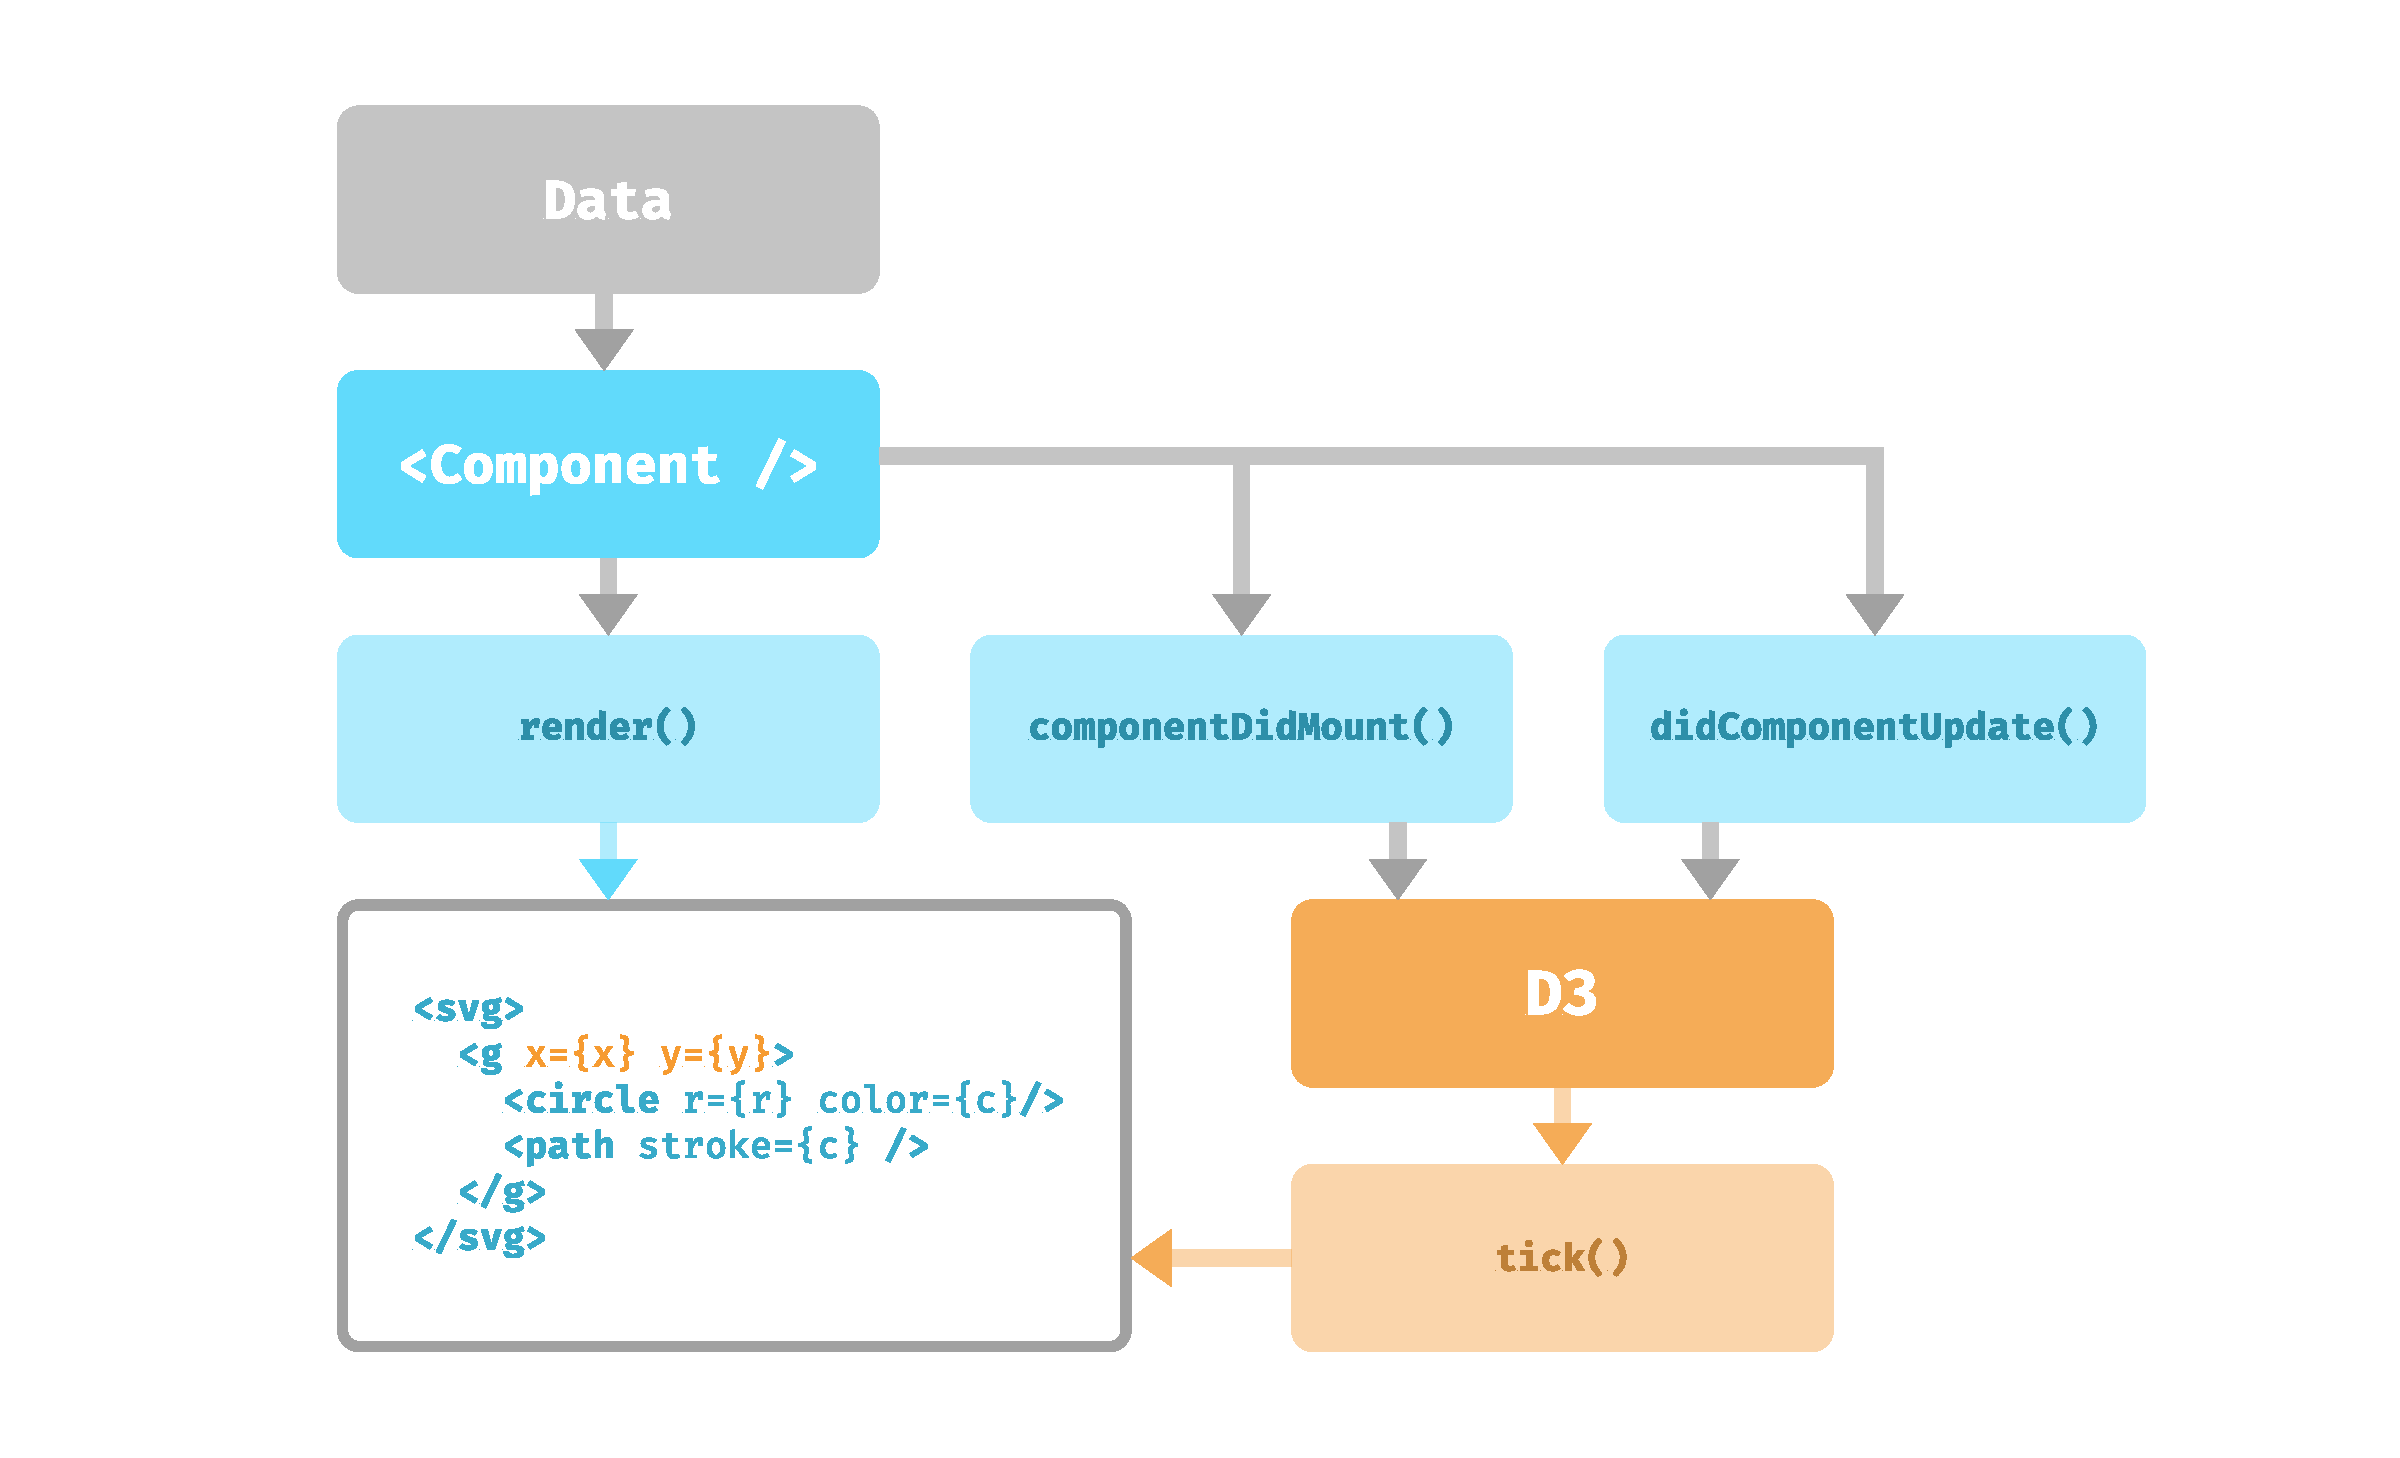
\includegraphics[scale=.6, trim= 4cm 0 4cm 0, clip, width=0.85\columnwidth]{impl003.pdf}
\caption{Pure \emph{React} force graph life cycle visualization.}
\label{fig:reactD3HybridLifeCycle}
\end{figure}

Last but not least, there is the \emph{D3} and \emph{React} hybrid force graph implementation. The prototype not only provides the developing experience of writing declarative \emph{React} code but also puts the complete feature set of \emph{D3} at the developers' disposal. The hybrid implementation makes it possible to handle the representational aspect of the simulation via \emph{React} and let \emph{D3} not only calculate but also manipulate the DOM node positions of the individual nodes and links in the force graph. Figure~\ref{fig:reactD3HybridLifeCycle} demonstrates via color coding what parts of the DOM content are handled by \emph{React} and \emph{D3}. 

The way the prototype achieves the previously mentioned functionality is that the \emph{D3} force simulation is constructed \emph{after} the hybrid \emph{React} component is initialized and mounted. As in the other two prototypes, all force data is passed into the hybrid force graph component via props from the parent component. \emph{React} renders the nodes and links which are represented in the props' data and after the render phase has been passed, the data is then handed to \emph{D3} via the \texttt{componentDidUpdate()} life cycle method. \emph{D3} selects the already committed DOM nodes and applies the internally calculated force position data. Figure~\ref{fig:reactD3HybridLifeCycle} demonstrates how only post render phase life cycle methods are used to pass data to \emph{D3}.

As described in chapter~\ref{cha:react}, during the component's render phase the reconciliation algorithm compares newly applied data of the component's state or props with the virtual DOM and then decides which DOM nodes need to be committed to or removed from the DOM. Once the simulation data updates via a prop update from the parent component, some nodes or links, therefore, might be added, changed or could just be removed, if they are non-existent anymore in the new version of the applied data.

The most important aspect of the hybrid prototype is that \emph{D3} selects already existing DOM nodes and connects them to the current force simulation data. Since the selection process is executed in \emph{React's} commit phase, \emph{D3} can read the up to date version of the DOM. As described in chapter~\ref{cha:react}, reading or manipulating the DOM in the commit phase guarantees the DOM to be a representation of the component's current state and data. Therefore \emph{D3's} selection happens \emph{after} the render phase to always apply its selection to the most recent version of the DOM.

\subsubsection{Implementation Details}

As the name of the component already reveals, the implementation of the hybrid prototype is a combination of the previous two prototypes. The initialization of the hybrid graph component also looks very similar to the initialization on line~\ref{line:buildForceSimulation} in the code snippet in program~\ref{prog:pureD3InitFn}. The only difference in the hybrid implementation is that the hybrid simulation type is passed to the builder function. A very notable difference to the pure \emph{React} component is that the initializer function is called in the \texttt{componentDidMount()} life cycle method, not in the component's constructor. As described before in the introduction of section~\ref{sub:D3AndReactHybrid}, the component needs to be in the commit phase for \emph{D3} being able to hook into already committed DOM nodes.

As described in section~\ref{sub:projectSetup}, the \texttt{buildForceSimulation()} function is very important to ensure every prototype the same \emph{D3} force simulation object. Any changes in given option parameters yield a different simulation of course, but the builder function is an idempotent function. If every prototype calls the builder function with the same force simulation option parameters, the method always returns the same simulation for every prototype. Like the other prototypes, the hybrid implementation of course also uses the force simulation builder function.

In contrast to the other prototypes, updating the hybrid graph component is quite simple. The code snippet in program~\ref{prog:hybridUpdateHandler} shows that the \texttt{componentDidUpdate()} life cycle method just calls the updater function that was obtained from the \texttt{build\-Force\-Simulation()} call. Since \emph{D3} handles the positioning of the nodes, updates in the components simulation data have to be passed to \emph{D3} to update its force calculation. While the pure \emph{React} prototype has to pass a complete render-cycle multiple times a second, the hybrid component only updates, if the parent container passes some new simulation data. As a consequence, the hybrid component can be rendered multiple times by the parent container but prevents itself from updating via implementing the \texttt{shouldComponentUpdate()} life cycle method.

\begin{program}
\caption{Component update handler of the hybrid force graph prototype.}
\label{prog:hybridUpdateHandler}
\begin{JsCode}
componentDidUpdate() {
  this.updateSimulation(this.extractSimUpdateParams())
}
\end{JsCode}
\end{program}

The tick handler, on the other hand, contains a few \emph{D3} specific instructions to display the current force simulation state. As mentioned before, the hybrid component makes \emph{D3} responsible for positioning the DOM nodes correctly according to the current simulation data. Line~\ref{line:hybridTickHhandler} in program~\ref{prog:hybridTickHandler} demonstrates, how the tick handler works in the hybrid prototype. To enable users of the component to pass custom simulation handlers, the node and link handlers are extracted from the props of the component first. If they are set from the parent container, they are utilized to handle the simulation tick. Otherwise the standard tick handlers on lines~\ref{line:applyNodeTick} and~\ref{line:applyLinkTick} are used. More information on how to customize the usage of the hybrid component can be read in chapter~\ref{cha:opensource} later on.

\begin{program}
\caption{Simulation tick handler of the hybrid force graph prototype.}
\label{prog:hybridTickHandler}
\begin{JsCode}
applyNodeTick = (nodeSel) => nodeSel.attr('cx', (d) => d.x).attr('cy', (d) => d.y) /+\label{line:applyNodeTick}+/
applyLinkTick = (linkSel) => linkSel.attr('d', this.getLinkPath) /+\label{line:applyLinkTick}+/

ticked = () => { /+\label{line:hybridTickHhandler}+/
  const { nodeTickHandler, linkTickHandler } = this.props

  nodeTickHandler /+\label{line:decideNodeTickHandler}+/
    ? nodeTickHandler(this.simulation.nodeSel)
    : this.applyNodeTick(this.simulation.nodeSel)

  linkTickHandler /+\label{line:decideLinkTickHandler}+/
    ? linkTickHandler(this.simulation.linkSel)
    : this.applyLinkTick(this.simulation.linkSel)
}
\end{JsCode}
\end{program}

Like the pure \emph{D3} prototype, the hybrid prototype also supports transitions. To achieve \emph{D3's} transition functionality, a library called \emph{react-move}---which can be found on its \emph{GitHub} page in~\cite{ReactMove}---provides the functionality for \emph{React} components. Because \emph{React} only renders its current state as a function of state, it is not possible to keep track of data throughout multiple render cycles. If, for example, a node with index "42" exists in render cycle one but not in render cycle two, there is no way for \emph{React} to know that there was a node with index "42" in the first render cycle. \emph{React} move provides an animation mechanism to tackle the previously mentioned problem. All of the simulation data is passed to the \emph{react-move} component inside the hybrid node component, which then keeps track of data changes via an internal system. Via animation hook functions the behaviors of entering, transitioning, and exiting nodes can be specified, which is similar to the \emph{D3} prototype. Information about the usage and how the \emph{react-move} library works internally can be found on the \emph{GitHub} project in~\cite{ReactMove}.


\subsubsection{Advantages}

The benefit of the hybrid implementation is that \emph{React} can handle the node and link representation. Writing \emph{React} code also implies that there are no disjointed code fragments of appending and removing components like in \emph{D3} code. Using \emph{React} components to render the force simulation nodes also implies that custom node components can be written and used in the force component, which makes the hybrid implementation highly versatile.

The rendering performance is probably close to a pure \emph{D3} implementation, as \emph{React} has to render the nodes for the simulation only once every data update. \emph{D3} then takes over by altering the positions on the actual DOM nodes via its internal ticking function. Technically there is no difference between rendering the initial nodes and links of a force graph via \emph{React} or \emph{D3} as the DOM nodes have to be committed nevertheless. \emph{D3's} force simulation tick cycles then directly alter the position attributes of the DOM SVG nodes. \emph{React} is agnostic of \emph{D3} being hooked into the DOM nodes, as the component only updates if the outside data changes. When the parent passes new simulation data, the simulation is fully updated in any case. Final numbers on performance are elaborated in chapter~\ref{cha:performance} though.

\subsubsection{Disadvantages}
\label{subsub:hybridDisadvantages}

A sig\-nifi\-cant disadvantage of the hybrid prototype is that it might be unclear to maintainers of the library that \emph{D3} handles the positions of the nodes and links and not \emph{React}. Of course, documenting the positioning aspect could be a solution to the problem. Writing proper documentation is not only time but also resource consuming for maintainers. New maintainers of the library would have to completely understand how the hybrid combination of \emph{React} and \emph{D3} works to start being productive on the library.

\section{Comparison of the Different Proposed Prototypes}

When comparing the prototypes, an essential aspect is to understand, which technology renders what aspects of the simulation's nodes and links. Looking at the pure \emph{D3} prototype, \emph{React} only renders the base SVG element so \emph{D3} can hook into the SVG base node and build up its simulation. The pure \emph{React} prototype, on the other hand, renders the complete DOM node tree of the whole simulation, including the nodes' and links' positions. Last but not least, the hybrid prototype introduces a mixed rendering strategy, where \emph{React} renders the whole DOM node tree, but \emph{D3} selects the already rendered nodes and only manipulates their positions.

The performance of the pure \emph{D3} prototype should act as a baseline for testing the other prototypes, as the whole simulation is handled by native \emph{D3} code. The pure \emph{React} prototype has to iterate a whole \emph{React} render cycle on each simulation tick, which technically is performing worse than letting \emph{D3} manipulate the DOM nodes directly. Therefore the hybrid prototype takes advantage of both worlds by leaving the expensive calculations and node position manipulations to \emph{D3} while Rendering the nodes with declarative \emph{React} code.

Looking at the figures~\ref{fig:pureD3Lifecycle},~\ref{fig:pureReactLifecycle}, and~\ref{fig:reactD3HybridLifeCycle} again, they might appear to be quite similar. There are some subtle differences which make big differences though. Even though all prototypes mostly use two life cycle methods, it is of utmost importance to recall in which component life cycle phase the methods are called though. Figure~\ref{fig:reactLifecycleMethods} can help to look up all common life cycle methods again. While the pure \emph{D3} and hybrid prototype pass the simulation to \emph{D3} only in the commit phase, the pure \emph{React} prototype has to pass its data to \emph{D3} in the render phase.

\section{Prototype Storybook}

\begin{figure}
  \centering
  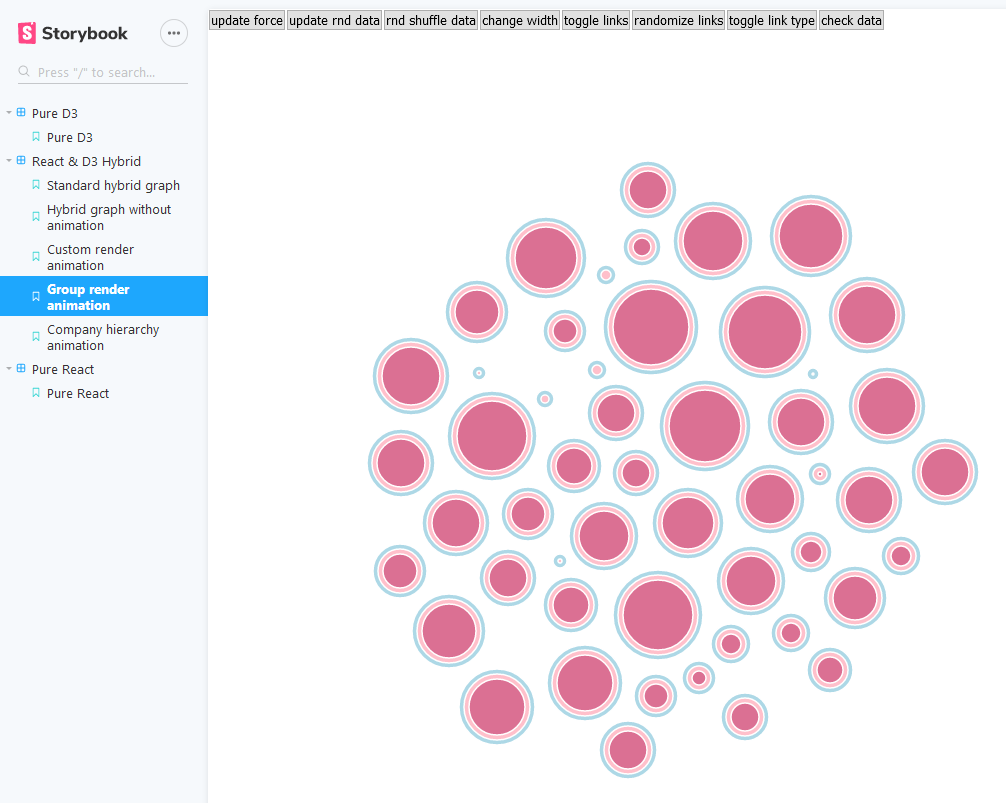
\includegraphics[width=0.89\columnwidth]{reactd3story}
  \caption{\emph{React} Storybook currently showing the hybrid prototype.}
  \label{fig:reactD3stroy}
\end{figure}

The thesis project furthermore contains one additional aspect that makes it quite easy to compare and test out all available prototypes. A community project called \emph{Storybook} was utilized to compare and present the prototype results. The \emph{GitHub} page in~\cite{ReactStorybook} explains the \emph{Storybook} software as a development environment for UI components. The library lets developers build component browsers for their projects which showcase the project's components in so-called "stories." A story is a self-contained page which renders a component with a pre-applied configuration and state. In the case of the thesis project, the \emph{Storybook} library was used to present all three prototypes in action and to make them interactive and browsable.

Figure~\ref{fig:reactD3stroy} shows a visualization of the \emph{Storybook}, which was developed for the thesis project. Users can select a prototype and a particular configuration from the sidebar and view the result in the main content section. All components are rendered inside a state container that provides data manipulation functionalities. For instance, via a simple click, the force data can be updated, links can be toggled, data or links can be shuffled and so on. All possible data manipulation functions can be seen in figure~\ref{fig:reactD3stroy} on top of the component section.

\section{Conclusion}

All in all, each prototype has an interesting implementation on its own. The implmentation phase of the thesis project showed that every prototype has certain advantages and disadvantages. The question of which prototype is the best is a subjective decision in the end. An aspect that can be measured though is performance. Chapter~\ref{cha:performance} shows how the particular prototypes perform in comparison to each other. As letting other developers profit from the findings of this master project is desired, the hybrid prototype will be an open source project in the near future. More information about the plans of making the newly invented hybrid prototype open source can be read in chapter~\ref{cha:opensource}.